% this file is called up by thesis.tex
% content in this file will be fed into the main document

\chapter{Chat Discourse Segmentation and Boundary Identification} % top level followed by section, subsection
\label{ch:TM}

\begin{textsl}
{\small Collaborative chat tools and large text corpora are ubiquitous in today's world of real-time communication. As micro teams and start-ups adopt such tools, there is a need to understand the meaning (even at a high level) of chat conversations within collaborative teams. In this study, we propose a technique to segment chat conversations to increase the number of words available (19\% on average) for text mining purposes. Using an open source dataset, we answer the question of whether having more words available for text mining can produce more useful information to the end user. Our technique can help micro-teams and start-ups with limited resources to efficiently model their conversations to afford a higher degree of readability and comprehension. }
\end{textsl}

\vspace*{1cm}

%\adjustmtc

%\minitoc
% ----------------------- contents from here ------------------------


% % % % % % % % % % % % % % % % % % % % % % % % % % % % % % % % % % % % % % % % % % % % % % % % % % % % % %
%---------------------------------------- INTRODUCTION ----------------------------------------------------
% % % % % % % % % % % % % % % % % % % % % % % % % % % % % % % % % % % % % % % % % % % % % % % % % % % % % %
\section{Introduction}
We live in an information age, and consumer-based services and applications generate more text-based data. As we embrace both collaborative and social communication, we converse more often via text-based communication \cite{talkmore2015} \cite{textstats2016}.  For both business and recreational purposes real-time chat discourse appears to be part and parcel of our lives. 

However, for businesses irrespective of size, using such collaborative and social means of communication, can be an overwhelming experience \cite{huffpost2016}. This is due in part to the large volumes of text-based data that are generated by such applications and services. Recent studies have shown that almost 350,000 tweets are created every minute of every day. Globally 2.5 quintillion bytes of data are produced \cite{venturebeat2016}. The growth in social media messaging is not confined to tweet messages. A recent study \cite{socmsg2017} by the Harvard business school has shown that over 2.5 billion users communicate with at least one messaging app (e.g. WhatsApp, Facebook). This figure will rise to 3.6 billion users in the next few years. Therefore, for this study, we consider techniques that may help teams make sense of their message based data.   

Topic modelling is a frequently used process to discover semantic structure within a text corpus. Topic modelling and text mining are used across multiple disciplines \cite{tmvalue2017} as a vehicle to grow business insights \cite{dti2017}. For example, if a business can mine customer feedback on a particular product or service this information may prove valuable \cite{softadvice2015}. One of the recommendations when employing text mining/topic modelling techniques is that the more data available for analysis, the better the overall results. However, even in the age of big data, practitioners may have a requirement to text mine a single conversation or small text corpus to infer meaning. 

In this paper, we propose a framework that both micro teams and SMEs can use to deliver a significant level of topic modelling terms, from real-time chat discourse data, while utilising their limited resource cohort. The core idea of this framework is for topic mining practitioners to partition their conversations using a novel technique. Such a method can provide a higher number of words (19\% on average) for topic summarisation tooling. For small teams with a limited pool of test resources, leveraging such segmentation techniques can provide not only more words for text mining but an improved level of readability than using an entire message corpus alone.

This paper contains research conducted on an open-source real-time chat corpus. Through the study of this dataset we investigate a) If by partitioning messages based on their inter-arrival time, can a more significant number of distinct words be returned for use by topic modelling software? b) Does a higher number of words provide a level of readability that is easier for humans to comprehend? c) Can we use the results of this work to predict an optimal topic cluster size? Using the results of this study for our framework, a topic mining solution can be developed to provide an enhanced level of understanding for small message corpora.

\section{Case study 7 - Chat discourse segmentation}

Topic modelling and text mining of social media/collaboration messaging have been shown to provide insight into the subjects people discuss as part of their online communication. By segmenting instant message text in a novel way, before topic modelling, we demonstrate how a higher degree of understanding can be achieved by the results of topic model outputs. 

For this study, we topic modelled three complete chat conservations from an open source Ubuntu developer IRC channel \cite{irclogs}. For each conversation, IRC messages were read, we noted an initial salutation, a valediction and a grouped topic discussed in-between the greeting and farewell messages. For this study, only conversations with related topic content were considered. We note that chat conversations with mixed chat messages (i.e. `entangled chat conversations') are beyond the scope of this study and will not be considered here. 

\begin {table}[]
\caption {Summary of Dataset Conversation Metrics} 
\label{tab:chapt7_study1_tab1}
\begin{center}
\begin{tabular}{| p{5.5cm} | p{1.5cm} | p{1.5cm} | p{1.5cm} |} \hline
\textbf{Metric} & \textbf{Chat 1} & \textbf{Chat 2} & \textbf{Chat 3} 
\\ \hline Total Messages & \multicolumn{0}{|r|}{46} & \multicolumn{0}{|r|}{70} & \multicolumn{0}{|r|}{59}
\\ \hline Total Words & \multicolumn{0}{|r|}{292} & \multicolumn{0}{|r|}{436} & \multicolumn{0}{|r|}{484}
\\ \hline Non-Stopped Words & \multicolumn{0}{|r|}{158} & \multicolumn{0}{|r|}{239} & \multicolumn{0}{|r|}{262}
\\ \hline Distinct Non-Stopped words & \multicolumn{0}{|r|}{111} & \multicolumn{0}{|r|}{168} & \multicolumn{0}{|r|}{186}
\\ \hline \% Words for analysis & \multicolumn{0}{|r|}{38} & \multicolumn{0}{|r|}{39} & \multicolumn{0}{|r|}{38} 
\\ \hline
\end{tabular}
\end{center}
\end{table}


Table~\ref{tab:chapt7_study1_tab1} provides a summary of the number of total words, the non-stopped words, the distinct non-stopped words and the percentage of words available for analysis. 

This study aims to answer the following questions. First, can we segment a chat conversation in such a way as to provide a greater number of distinct words for topic modelling algorithms? Second, if a reasonable segmentation method can be found, is the output from a topic model easier to infer meaning, then modelling the entire conversation alone? Third, is there a relationship between the topic modelling cluster size and the number of words Input/Output from topic modelling? 

\subsection{Conversation segmentation}

A question for practitioners of topic modelling is, how can we maximise the number of words for analysis? We know from prior research that text mining algorithms that some form of text pre-processing is required prior to topic modelling. Pre-processing may include at least one of the following: Tokenisation, stop words removal, stemming and lemmatisation. The removal of words as part of this pre-processing step usually is not an issue for a large text corpus, due to the number of words available. In the case of small text corpora, the problem may be more acute. For our study, stemming and lemmatisation was not conducted.

We recorded the inter-arrival time of instant message posts within the Ubuntu IRC channel, and grouped messages by short and long inter-arrival times. For successive messages with a zero minute inter-arrival time, we define this collection of messages as a burst. For messages with a one minute or greater inter-arrival time, we define this group of messages as a reflection. We then perform text mining on each burst and reflection period and then aggregate the output terms. For topic text mining, we used the tool Biterm, which is suited to modelling small text corpora.

\subsection{Topic modelling comprehension}

\begin {table}[]
\caption {Summary of Differences between Questionnaire Samples} 
\label{tab:chapt7_study1_tab1a}
\begin{center}
\begin{tabular}{| p{2.5cm} | p{6.9cm}  |} \hline 
\textbf{Sample 1} & Entire chat - Topic Modelled  
\\ \hline  \textbf{Sample 2} & Burst \& Reflections - Topic Modelled
\\ \hline  \textbf{Sample 3} & Entire chat - Stop words removed 
\\ \hline  \textbf{Sample 4} & Entire chat - No text pre-processing 
\\ \hline
\end{tabular}
\end{center}
\end{table}

After a conversation has been a) segmented into burst and reflection periods, b) these periods topic modelled and c) the results aggregated, we consider the efficacy of the output. 

We accept that the terms output from a topic model algorithm is not explicitly designed for a readable summary. Instead, they are designed to give a user an indication of the terms used in a text corpus. Nevertheless of interest is how a user can understand the output of text mining. Our approach is to prepare four sets of text as follows; 1) each conversation is modelled with Biterm (as a whole) and the mined terms output into a single collection, 2) the bursts and reflections from each conversation are modelled individually, the terms are then aggregated into a single collection, 3) each conversation with the stop words removed and 4) the raw conversation (i.e. without any pre-processing). Table ~\ref{tab:chapt7_study1_tab1a} summarises the level of pre-processing conducted for each sample.

We then asked twenty four test subjects to summarise each of the four text sets belonging to a single conversation. Additionally, we asked each participant to comment on which of the four text sets was easiest to summarise. Next, we asked each subject, whether they felt set one (all terms topic modelled) or set two (bursts and reflections topic modelled) was most natural to summarise. Finally, we asked each subject to describe why they felt the text set chosen in the second question was easiest to summarise. Results of a meta-study on sample sizes for qualitative studies \cite{qualsample} show there is variability in sample size depending on the subject domain. For our questionnaire, twenty-four individuals were selected, and each conversation was randomly distributed among the users.

Finally we compared the readability of every text set for each conversation using a number of known readability tests such as; Dale-Chall \cite{dale1948formula}, Coleman-Liau \cite{coleman1975computer}, Flesch-Kincaid \cite{kincaid1975derivation} and Gunning Fog \cite{gunning1952technique}. 

\subsection{Term cluster size prediction}

Topic modelling algorithms use a unique set of words from a corpus for analysis. Also, we know that the process of text mining may be, in part non-deterministic. In other words, random sampling is often used to generate a term list. One of the goals of text mining is to ensure that a sufficient number of words are output in each topic cluster. The intuition is that the more unique words that are provided, perhaps the easier the output will be to understand.

Biterm, outputs topic mined terms as `topic clusters'. Each cluster has a maximum size of ten terms. If one hundred words are input for analysis, the intuition is that ten clusters will be output with a ten distinct words. However, due to the underlying random nature of the sampling algorithm used, this is not always the case. Therefore, it is necessary to use a range of cluster sizes to obtain the optimal number of terms. We define `optimal output words' as the number of words that closely matches the number of words used for Biterm analysis. We define the `optimal \# clusters', as the smallest number of clusters that contains the optimal output words.

Linear regression is a method to determine the relationship between two or more variables where one variable is dependent, and the additional variables are independent. A hypothesis test (are two or variables correlated) is conducted, and a p-value is computed. Depending on the size of the p-value, the hypothesis of a relationship/no relationship can be accepted or rejected. We used the lm function found in the base R package \cite{lmR} and performed a linear regression test.

We will use linear regression to explore the relationship between the number of unique words input, the Biterm cluster size and the unique terms output. For example, if we model the unique words input to Biterm, the cluster size that provides the unique optimal set of terms and the count of these text mined terms, a linear model could be used to predict optimal term cluster size.

\subsection{Limitations of dataset}

The dataset has some practical limitations, which are now discussed. The process of aggregating chat messages into a cohesive conversation is a subjective one. Every effort was made to assign messages to their most appropriate thread. We recognise that the process is subjective. Additionally, the post times for the Ubuntu chat were measured in hours and minutes only. As a result, we defined our burst and reflection period as timed in zero and one minute or greater priors respectively. 

The chat conversations that form part of this case study are from an Ubuntu IRC developer channel. While we hope these examples will be representative of technical discussion channels, it seems unlikely they will be typical of all types of channels.

\section{Results}

We now explore the results of our analysis.

\subsection{Conversation segmentation}

\begin {table}[]
\caption {Summary of Text Mining Analysis: Entire Conversations Vs Burst and Reflections} 
\label{tab:chapt7_study1_tab2}
\begin{center}
\begin{tabular}{| p{6.8cm} | p{1.5cm} | p{1.5cm} | p{1.5cm} |} \hline \textbf{Metric} & \textbf{Chat 1} & \textbf{Chat 2} & \textbf{Chat 3} 
\\ \hline Total words & \multicolumn{0}{|r|}{292} & \multicolumn{0}{|r|}{436} & \multicolumn{0}{|r|}{484} 
\\ \hline Non-stopped words & \multicolumn{0}{|r|}{158} & \multicolumn{0}{|r|}{239} & \multicolumn{0}{|r|}{262} 
\\ \hline Distinct non-stopped words & \multicolumn{0}{|r|}{111} & \multicolumn{0}{|r|}{168} & \multicolumn{0}{|r|}{186}
\\ \hline Distinct non-stopped terms output & \multicolumn{0}{|r|}{96} & \multicolumn{0}{|r|}{129} & \multicolumn{0}{|r|}{143} 
\\ \hline \# Words not analysed & \multicolumn{0}{|r|}{196} & \multicolumn{0}{|r|}{307} & \multicolumn{0}{|r|}{341} 
\\ \hline \% Words for analysis & \multicolumn{0}{|r|}{38} & \multicolumn{0}{|r|}{39} & \multicolumn{0}{|r|}{38} 
\\ \hline \% Actual terms output & \multicolumn{0}{|r|}{33} & \multicolumn{0}{|r|}{30} & \multicolumn{0}{|r|}{30} 
\\ \hline & & & 
\\ \hline Total burst words & \multicolumn{0}{|r|}{185} & \multicolumn{0}{|r|}{226} & \multicolumn{0}{|r|}{287} 
\\ \hline Non-stopped burst words & \multicolumn{0}{|r|}{98} & \multicolumn{0}{|r|}{143} & \multicolumn{0}{|r|}{163} 
\\ \hline Distinct non-stopped burst words & \multicolumn{0}{|r|}{91} & \multicolumn{0}{|r|}{118} & \multicolumn{0}{|r|}{154} 
\\ \hline Distinct non-stopped terms output & \multicolumn{0}{|r|}{87} & \multicolumn{0}{|r|}{118} & \multicolumn{0}{|r|}{145} 
\\ \hline \# Burst words not analysed & \multicolumn{0}{|r|}{94} & \multicolumn{0}{|r|}{108} & \multicolumn{0}{|r|}{142} 
\\ \hline \# Bursts & \multicolumn{0}{|r|}{7} & \multicolumn{0}{|r|}{11} & \multicolumn{0}{|r|}{8} 
\\ \hline \% Words for analysis & \multicolumn{0}{|r|}{49} & \multicolumn{0}{|r|}{52} & \multicolumn{0}{|r|}{54} 
\\ \hline \% Actual terms output & \multicolumn{0}{|r|}{47} & \multicolumn{0}{|r|}{52} & \multicolumn{0}{|r|}{51} 
\\ \hline & & & 
\\ \hline Total Reflection words & \multicolumn{0}{|r|}{107} & \multicolumn{0}{|r|}{210} & \multicolumn{0}{|r|}{197} 
\\ \hline Non-stopped reflection words & \multicolumn{0}{|r|}{61} & \multicolumn{0}{|r|}{99} & \multicolumn{0}{|r|}{99} 
\\ \hline Distinct non-stopped reflection words & \multicolumn{0}{|r|}{60} & \multicolumn{0}{|r|}{95} & \multicolumn{0}{|r|}{94} 
\\ \hline Distinct non-stopped terms output & \multicolumn{0}{|r|}{60} & \multicolumn{0}{|r|}{93} & \multicolumn{0}{|r|}{94} 
\\ \hline \# Reflection words not analysed & \multicolumn{0}{|r|}{47} & \multicolumn{0}{|r|}{115} & \multicolumn{0}{|r|}{103} 
\\ \hline \# Reflections & \multicolumn{0}{|r|}{7} & \multicolumn{0}{|r|}{12} & \multicolumn{0}{|r|}{9} 
\\ \hline \% Words for analysis & \multicolumn{0}{|r|}{56} & \multicolumn{0}{|r|}{45} & \multicolumn{0}{|r|}{48} 
\\ \hline \% Actual terms output & \multicolumn{0}{|r|}{56} & \multicolumn{0}{|r|}{44} & \multicolumn{0}{|r|}{48} 
\\ \hline
\end{tabular}
\end{center}
\end{table}


Table \ref{tab:chapt7_study1_tab2} shows a summary of the topic modelling conducted on each of the three conversations. In the first experiment, the entire discussion was mined. In the second experiment, the burst and reflections were modelled separately. 

For conversation one, a total of 96 terms were output by Biterm when modelling the entire text, whereas 87 and 60 terms respectively were output from the burst and reflection analysis. A total of 51 (17\%) more terms were output from the combined burst and reflection analysis than modelling the entire conversation.

For conversation two, a total of 129 terms were output by Biterm, whereas 118 and 93 terms respectively were output from the burst and reflection analysis. A total of 82 (19\%) more terms were output from the combined burst and reflection analysis than modelling the entire conversation.

For conversation three, a total of 143 terms were output by Biterm, whereas 145 and 94 terms respectively were output from the burst and reflection topic mining. A total of 96 (20\%) more terms were output from the combined burst and reflection analysis than modelling the entire conversation.

\subsection{Topic modelling comprehension}

\begin {table}[]
\caption {Summary of Text Sample Questionnaire Answers (Q1 \& Q2)} 
\label{tab:chapt7_study1_tab3}
\begin{center}
\begin{tabular}{| p{3.5cm} | p{2cm} | p{2cm} | p{2cm} | p{2cm} |} \hline \textbf{Question} & \textbf{Sample 1 - Biterm (All text)} & \textbf{Sample 2 - Biterm (Burst \& Reflections)} & \textbf{Sample 3 - (Stop words removed)} & \textbf{Sample 4 - (Full text)} 
\\ \hline One: Of the 4 text samples, which sample did you find easier to summarise? (1/2/3 or 4) & 0 & 0 & 2 & 22
\\ \hline Two:  Of samples 1 and 2, which sample did you find easier to summarise? (1 or 2) & 0 & 24 & NA & NA
\\ \hline
\end{tabular}
\end{center}
\end{table}

Recalling the survey questions asked in section III part B: Of the four text samples, which sample did you find easier to summarise? And of samples 1 and 2, which sample did you find easier to summarise?
Table \ref{tab:chapt7_study1_tab3} shows a summary of the answers to the questions asked of the test subjects. Before the questionnaire, the subjects were asked to summarise the four samples. The questions were asked directly after the summarisation task. As we can see for question one, the majority of users found sample 4 easiest to summarise. For question two, the respondents answered unanimously in favour of sample 2.

\begin{figure}
\begin{center}
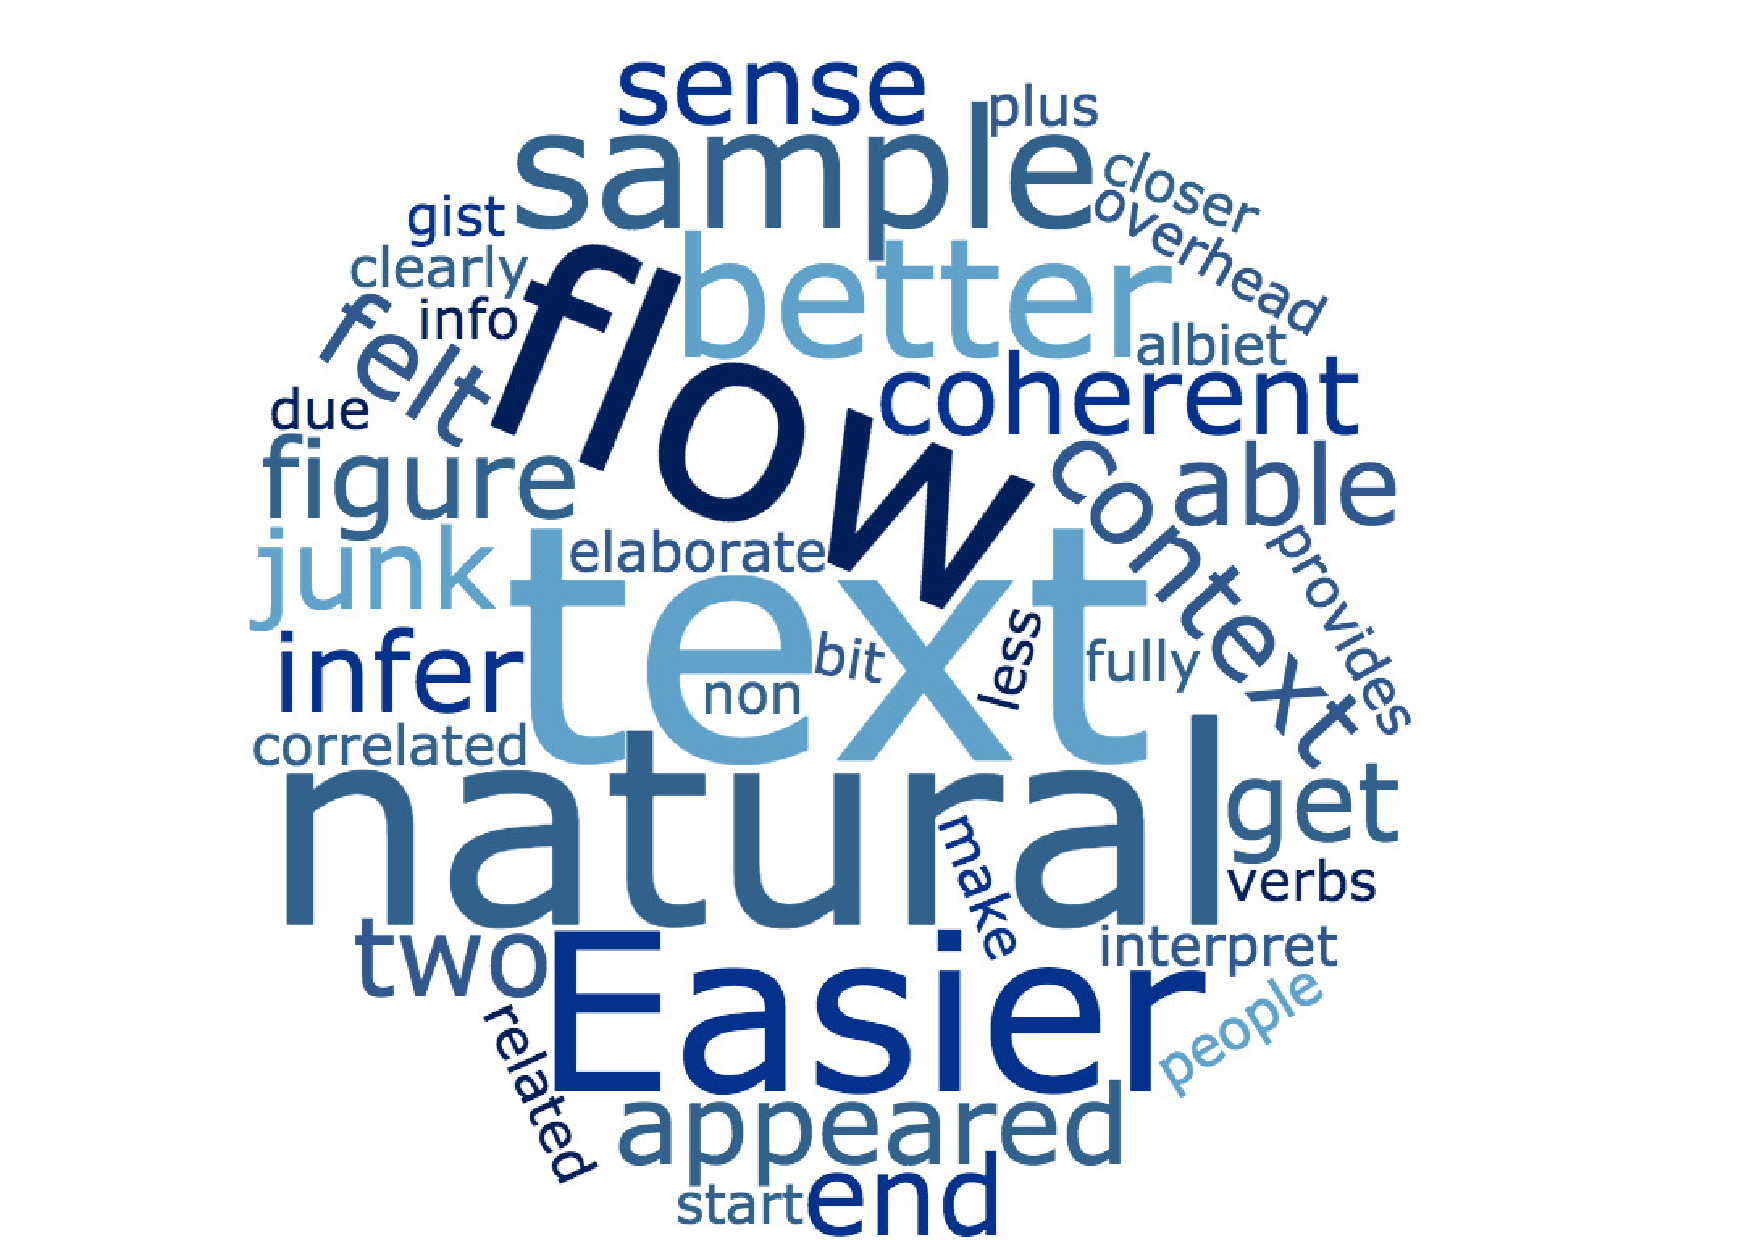
\includegraphics[height=9cm, width=14cm]{graphs/bundles/wordcloud_v2.pdf} 
\caption{Word Cloud of answers from survey question 3}
\end{center}
\label{fig:chapt7_study1_fig1}
\end{figure}

Question three asked: For the sample, you chose in question two, why did you find that text sample easier to summarise? Figure 7.1 shows a word cloud generated from the answers respondents provided. When stop words were removed, the following terms appeared most frequently: easier (8 times), text (6), words (5) and flow/natural/understand/words (all 5).

\begin{figure}
\begin{center}
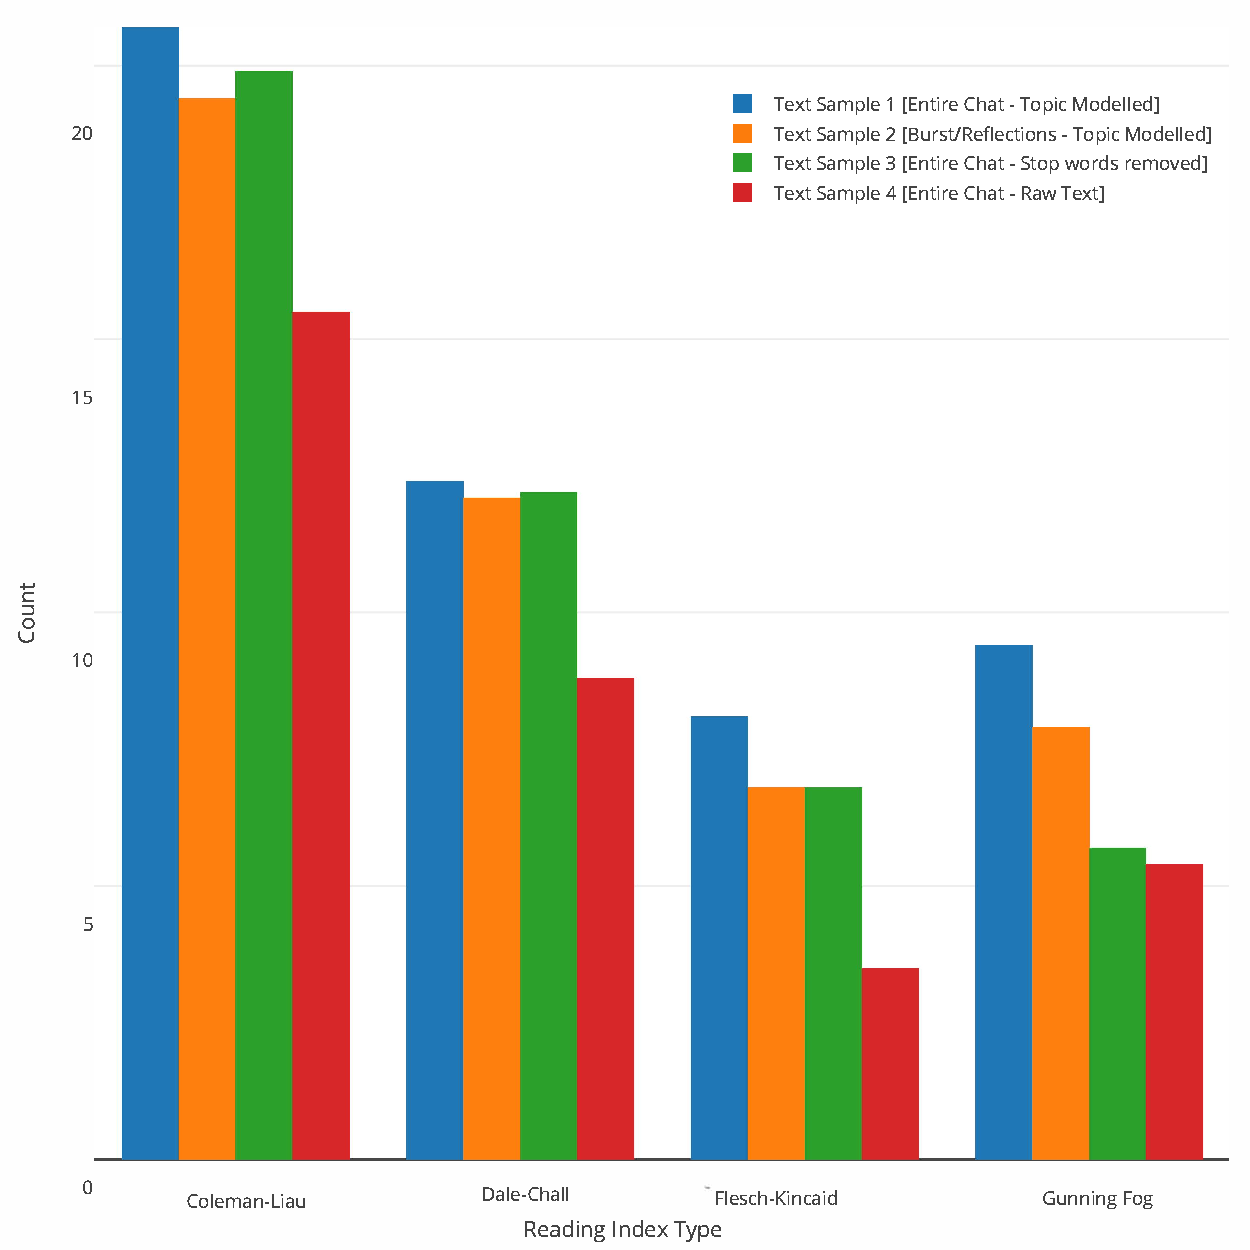
\includegraphics[height=9cm, width=14cm]{graphs/bundles/readindex1.pdf} 
\caption{Mean readability index score of each text sample}
\end{center}
\label{fig:chapt7_study1_fig2}
\end{figure}

To further understand the readability of text output from our topic mining experiments, we conducted some readability tests (Dale-Chall, Coleman-Liau, Flesch-Kincaid and Gunning Fog) against each of the four text samples for all three conversations. Figure 7.2 shows a bar chart of mean readability index scores. In all cases, a lower score indicates a more readable text sample. Intuitively we can see that text sample 1 had the highest score across all indices, and text sample 4 had a lowest. Text sample 2 had a lower index score than sample 1 in all readability tests.

% Thesis candidate only
\subsection{Term cluster size prediction}

Our third research question asked, ``Can we use the results of our topic modelling to predict an optimal topic bundle size?'' We mentioned previously that obtaining an optimal number of terms (i.e. an output number of distinct words that matches an input number of distinct words) from Biterm is an iterative process. 

For each burst, reflection and complete segment we topic modelled multiple cluster numbers to obtain the optimal number of distinct words. Once an optimal cluster size was found, the number of clusters was noted. We then used Linear regression to determine if there is a strong relationship between the number of distinct words output and the cluster size. In order words can we create a linear function to predict the number of topic clusters, if the optimal number of terms are known?


\begin {table}[]
\caption {Linear Regression Coefficient Table} 
\label{tab:chapt7_study1_tab4}
\begin{center}
\begin{tabular}{| p{3cm} | p{2.2cm} | p{2.2cm} | p{2.2cm} | p{2.2cm} |} \hline \textbf{Coefficients} & \textbf{Estimate} & \textbf{Std. Error} & \textbf{t value} & \textbf{Pr(\textgreater t)} 
\\ \hline (Intercept) & 0.934 & 0.122 & 7.606 & 3.45e-10
\\ \hline Optimal.Terms & 0.058 & 0.003 & 18.201 & \textless 2e-16
\\ \hline
\end{tabular}
\end{center}
\end{table}

Table \ref{tab:chapt7_study1_tab4} shows the output of the Linear regression analysis. We also note the following additional outputs;  Residual standard error: 0.818, Multiple R-squared:  0.855,	Adjusted R-squared:  0.853 and p-value: \textless 2.2e-16. From the output we can see that the equation to fit our linear model is as follows:

\begin{equation}
Number of Clusters = 0.934 + 0.058(Optimal.Terms)
\end{equation}

\begin{figure*}[]
\begin{center}
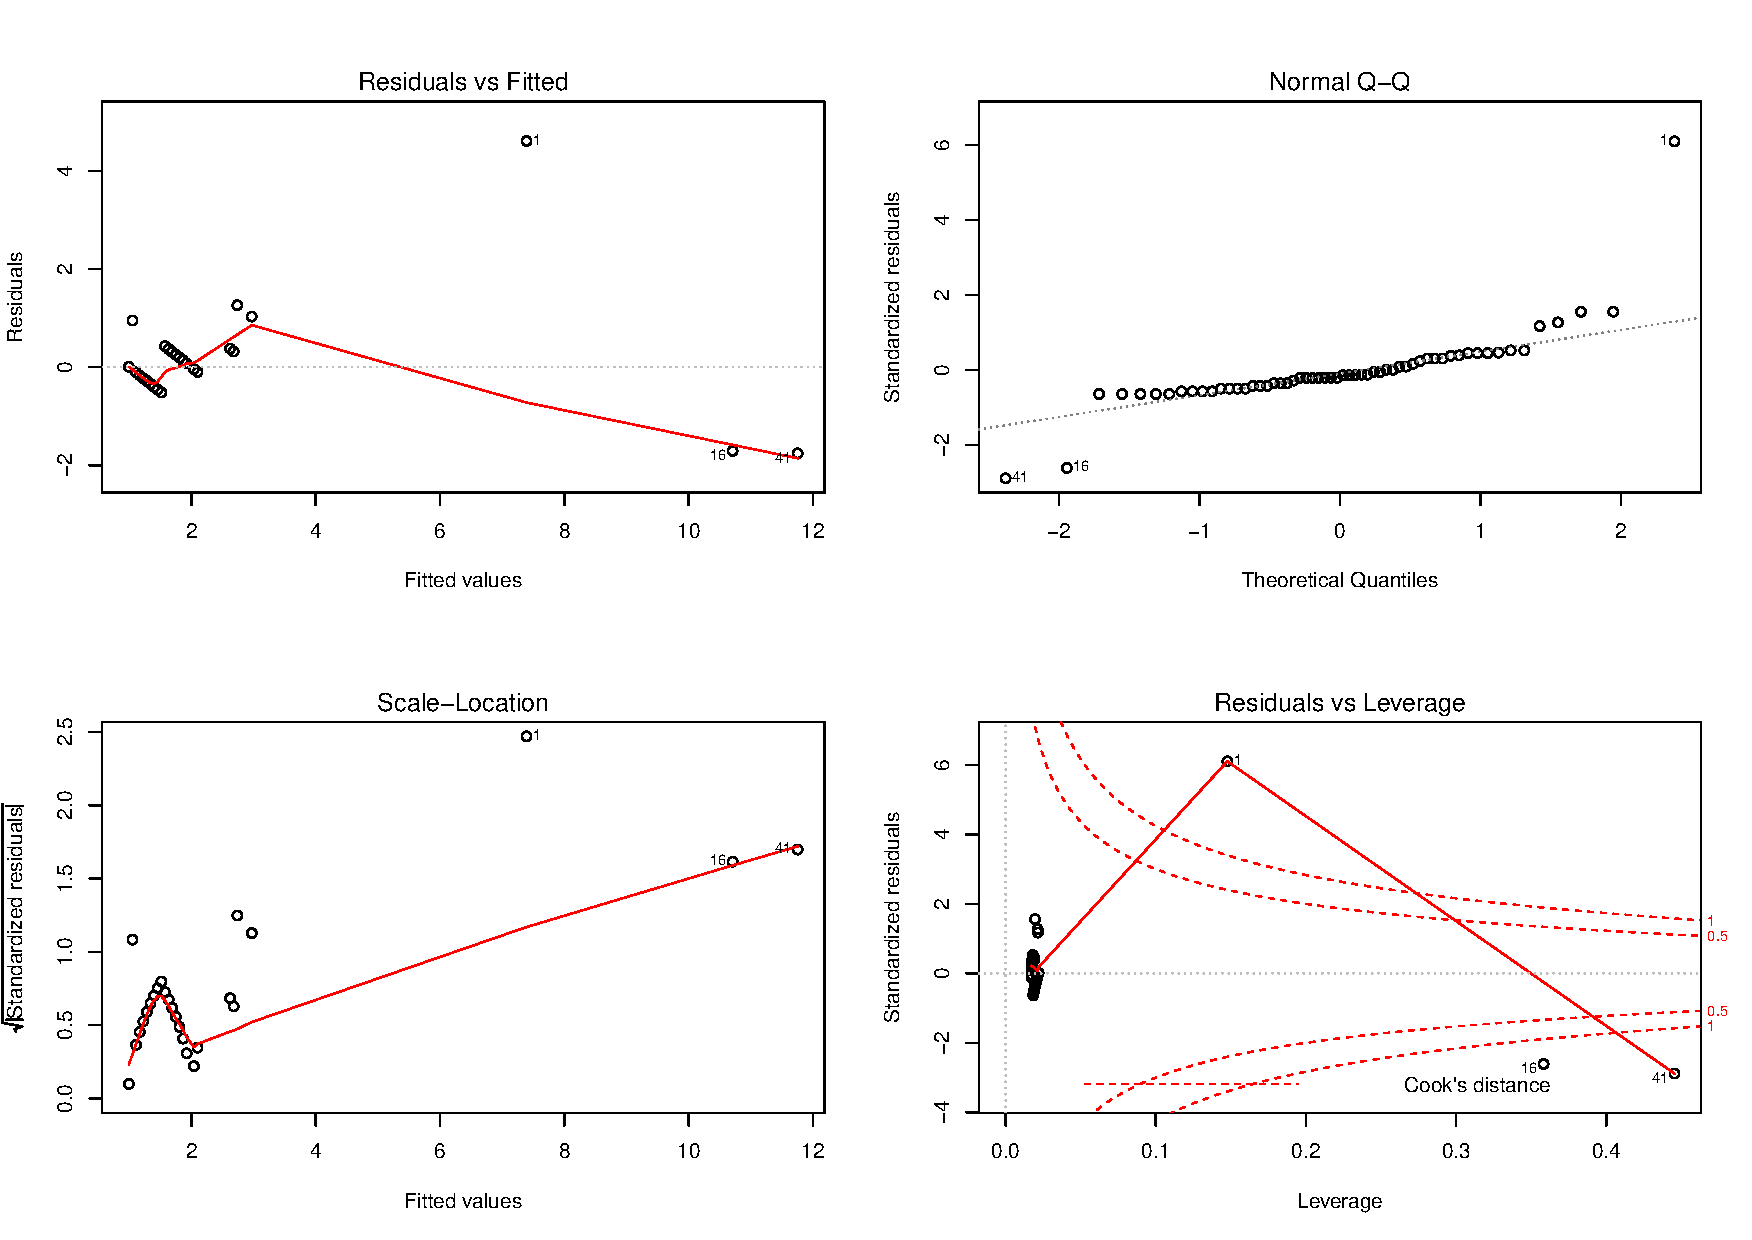
\includegraphics[height=9cm, width=14cm]{graphs/bundles/linear_fit1.pdf} 
\caption{Residuals Vs Fitted, Q-Q Plot, Scale-Location \& Residuals Vs Leverage}
\end{center}
\label{fig:chapt7_study1_fig3}
\end{figure*}

Figure 7.3 shows the four goodness-of-fit plots generated from our linear regression model. These plots are used in conjunction with the results of the Linear coefficients table to determine the suitability of the model. We shall discuss these results of the model in more detail in the next section.

\section{Discussion}

The following section provides deeper analysis and discussion of the results. In each section, references will be made to each research question asked in section 7.2.

\subsection{Conversation segmentation}

Our first research question asked, can we segment a chat conversation in such a way as to provide a higher number of unique words for topic modelling algorithms? Table \ref{tab:chapt7_study1_tab2} shows that the mean proportion of words available for analysis for topic modelling of an entire conversation is 38\%, this is due to the considerable number of stop words that are removed as part of pre-processing. Likewise, the mean number of terms output from Biterm is 31\% a reduction of 7\%.

Conversely, when both burst and reflections are aggregated, the mean proportion of terms available for analysis is 51\%. Furthermore, the mean proportion of terms output from Biterm is on average, 50\% a reduction of only 1\%.

There is evidence to suggest that segmenting conversations into shorter segments provides a greater number of words for topic analysis due to the lack of duplicate words found in each smaller segment. We note that stop words are removed irrespective of the segment size.

Some interesting points are raised by our analysis. When stop words are removed, duplicate occurrences of the same word are also discarded. However, in the case of a more substantial text corpus, some duplicate non-stop words remain, these words are ignored by text mining tools. We see this is not the case with burst and reflection text segments. In fact, for conversation 2, 143 non-stopped words were retained. A further 25 non-stop duplicate words were ignored. In all other cases, the number of duplicate words ignored by Biterm after stop words were removed was less than 10.

Furthermore, we observed that the number of burst and reflections created might have little significance on the number of terms output. Conversations 1 \& 3 had a similar number of segments (i.e. between 7 and 9), while conversation 2 had 11 burst and 12 reflections respectively. While no formal correlation tests were conducted, when we look at the segment size and the \% terms output, there seems little positive or negative relationship between the two variables.


\subsection{Topic modelling comprehension}

Our second research question asked: If a reasonable segmentation method can be found, is the output from a topic model easier to understand, than modelling the entire conversation alone? In other words, even if more words can be output as part of our improved segmentation technique, how does this translate into comprehension by both a human and for general readability. 

Table \ref{tab:chapt7_study1_tab3} summarises the answers to the first two survey questions asked by the 24 individuals who took part in our topic modelling comprehension experiment. Unsurprisingly we can see that the majority of respondents picked sample 4, as the easiest to summarise. The consensus was that with all words available and with grammar respected (to a degree) sample 4 was easiest to summarise for the majority. However, we note that two respondents picked sample 3 (stop words removed). The feedback from these two participants was that the samples with fewer words were easier to understand, this may be because these two individuals were not Ubuntu experts.

For survey question 2 the unanimous feedback from all users was that sample 2 was much easier to read than sample 1. A word cloud produced from the short answers provided, clearly indicate that a combination of our segmentation technique and Biterm preserved the natural flow of the conversation to the degree that it was easier to summarise the text sample than sample 1.

Turning to the readability tests conducted, we can see that sample 4 produced the lowest mean index score indicating that the unprocessed chat was the most readable based on the four tests conducted. Except for the Gunning Fog index, sample 2 had equal or lower readability scores than sample 3. 

It would be over-simplistic to state that when more words are available, it is easier for a human to understand a text segment based on a list of topic terms. However, it seems reasonable to assert that when more words are available and when words are placed in a similar order as to how they were typed, it is easier for humans to comprehend. What was interesting to note for short burst and reflection segments, (i.e. ten words or less) the input order of words was the same as the output terms produced by Biterm. That is to say the word at the start of the sentence had the highest log-likelihood value, while the word at the end of the sentence had the lowest log-likelihood value.

We note that the goal of this research question was not to provide a readable summary based on text mined terms. Instead, the goal was to assess the understanding of text samples to humans when varying degrees of topic mining is conducted. 

% Thesis candidate only
\subsection{Term cluster size prediction}

Our third research question asked: Can we use the results of our topic modelling experiments to predict the optimal cluster size? Previously, we discussed the problem of determining the number of clusters that will return the highest number of distinct words from the Biterm analysis. We also mentioned that the optimal cluster number could be obtained only by iteratively trying a range of sizes.

Table \ref{tab:chapt7_study1_tab4} provides the output of a linear regression experiment whereby we used the optimal terms to predict cluster size. The first point to note is that the p-value for optimal.terms was \textless2e-16, this figure indicts a strong regression effect. Additionally, we note that the multiple R-squared and adjusted R-squared values were 0.855 and 0.853. These values indicate the model is an excellent fit for our data.

Figure 7.3 depicts four goodness-of-fit plots to assess the goodness of fit of our model graphically. The residuals Vs fitted plot shows our model passes through the majority of fitted values quite well. It appears that a small number of points are outside the fitted line. The normal Q-Q plot shows the standardised residuals fitted against a normal distribution line. For the most part, almost all values fit the line. There are a number of exceptions, such as a few small and large residuals. This plot indicates the model would almost all values however there would be some uncertainty of fitted very small and very large values. Finally, three observations had leverage greater than 0.1.  

We mentioned previously that Biterm topic clusters contain ten terms, and that due to random variation of the tooling, it is not always possible to obtain the same level of distinct output terms as were input. For example, dividing the number of distinct words for analysis by ten and using this result as the optimal \# of clusters, does not provide the same amount of output words. However, we did not know to what degree of fit a linear model would provide. In our case, a good fit was obtained.

The main benefit such a linear model is as follows: Determining the optimal cluster size can be a time-consuming task, especially for large datasets. Even using a rule of thumb such as a `divide input distinct words by ten' as a starting point, multiple iterations of Biterm may be required. By using a linear model such as ours, the task of determining the optimal term cluster size may be expedited. 



% % % % % % % % % % % % % % % % % % % % % % % % % % % % % % % % % % % % % % % % % % % % % % % % % % % % % %
%------------------------------------------- CONCLUSIONS --------------------------------------------------
% % % % % % % % % % % % % % % % % % % % % % % % % % % % % % % % % % % % % % % % % % % % % % % % % % % % % %

\section{Conclusion}
The purpose of this study was to examine topic modelling for small text corpora (i.e. Instant message conversations). We found that by segmenting messages into periods of intense (bursts) and non-intense (reflections) communication that these segments, when used in conjunction with a text mining tool can be used to provide a higher number of output terms than modelling the entire corpus of messages at once. Furthermore, we found that the message inter-arrival time can be used to determine both burst and reflection periods.

We also found that the terms output from topic modelling bursts and reflection periods, when aggregated, is easier to understand than the text mined terms from the entire message corpus. Additionally, we saw that all four readability tests, topic modelled terms output from aggregated burst and reflection analysis have a lower readability index compared to terms mined from the entire corpus.

Finally, the relationship between optimal output words and the optimal \# clusters had a strong regression effect. In other words, we can use the optimal terms to predict the required number of topic clusters. This result can have a positive benefit for topic modelling practitioners, as it may reduce the iterative approach needed to find the number of topic clusters that produce the largest distinct number of words.

Both SMEs and micro-teams can use the above result to deliver high-value topic mining outputs from their group chat discourse. Teams can focus initially on a corpus-based approach for a particular channel/space. The advantage of a more extensive corpus approach is that topic modelled outputs can be assessed in context. Where words collations exist, this knowledge can be directly applied to place a higher value on terms generated from topic mining tools.

% ---------------------------------------------------------------------------
% ----------------------- end of thesis sub-document ------------------------
% ---------------------------------------------------------------------------
